% !TeX spellcheck = en_GB
\chapter{MEPS Snow Water Content}
\section{Ensemble Mean: Deterministic and First Perturbed Member}
%%% image 1h %%%%%%%%%%%%%%%%%%%%%%%%%%%%%%%%%%%%%
\begin{figure}[ht!]%\ContinuedFloat
	\centering
	% 21/12
	\begin{subfigure}[t]{\textwidth}
		\centering
		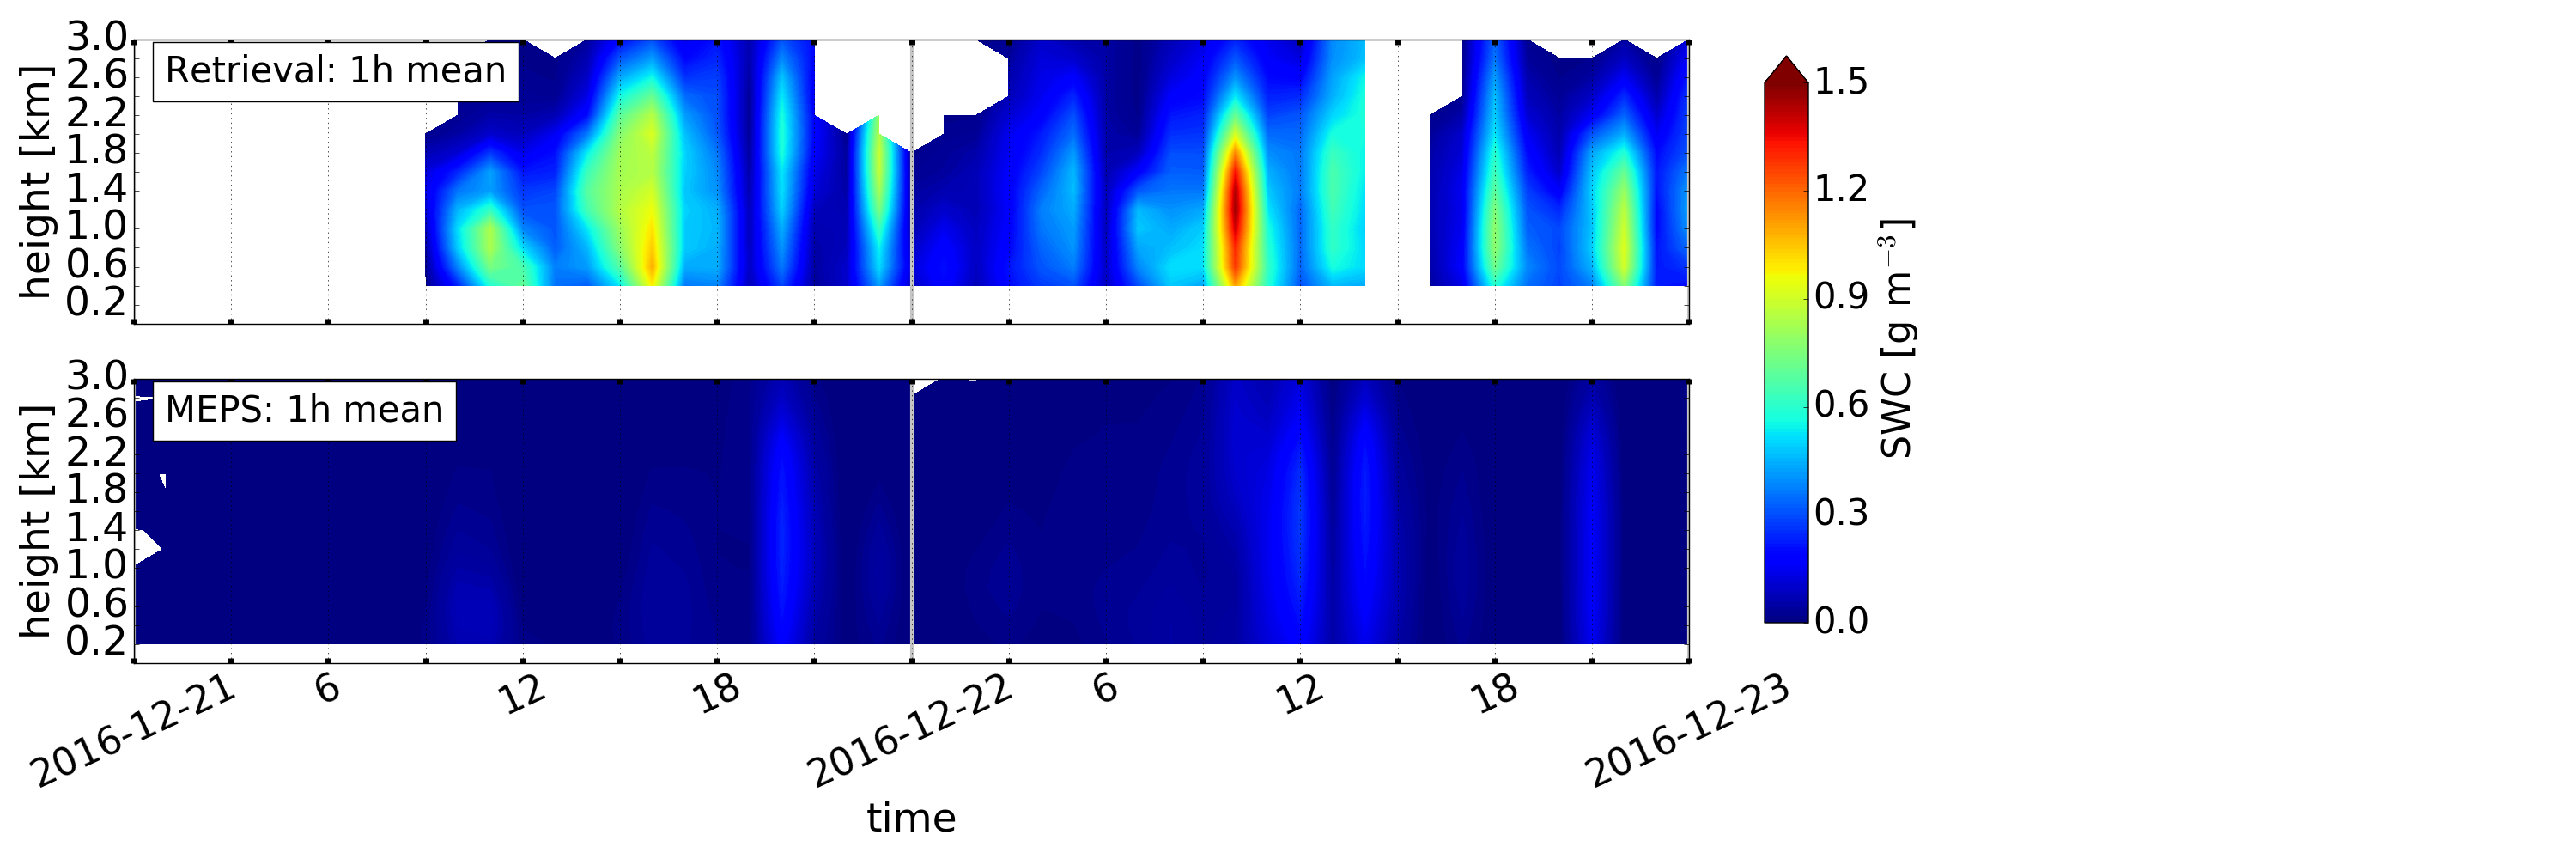
\includegraphics[trim={0.cm 0.8cm 19.cm 0.5cm},clip,width=0.9\textwidth]{./fig_vert_SWC_1h/20161221}
		\caption{}\label{fig:SWC1h:21}
	\end{subfigure}
	% 22/12
	\begin{subfigure}[t]{\textwidth}
		\centering
		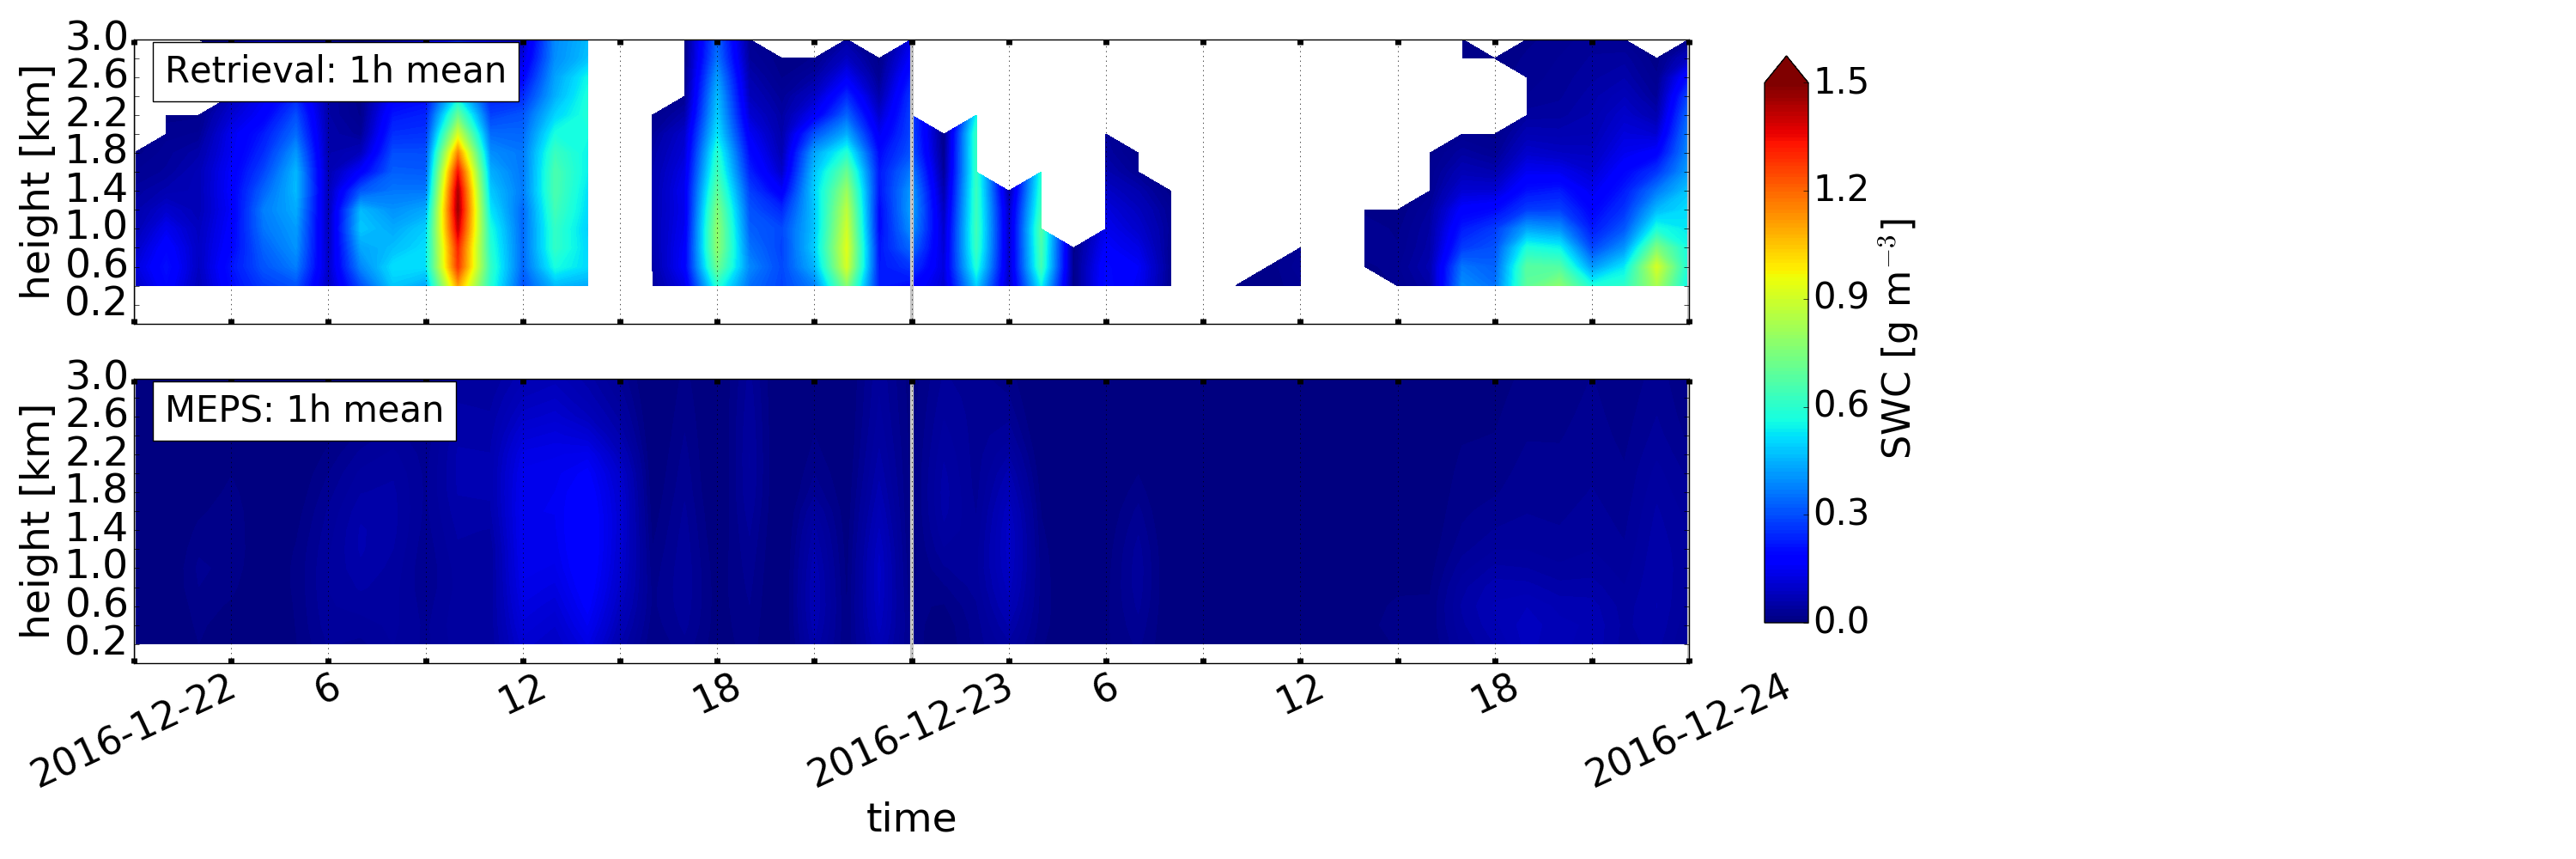
\includegraphics[trim={0.cm 0.8cm 19.cm 0.5cm},clip,width=0.9\textwidth]{./fig_vert_SWC_1h/20161222}
		\caption{}\label{fig:SWC1h:22}
	\end{subfigure}
	\caption{From upper to lower: Hourly averaged retrieved and hourly instantaneous ensemble mean forecast of deterministic and first ensemble member. Initialised \SIlist{21;22}{\dec} at \SI{0}{\UTC}. Shading according to the colour-bar. }\label{fig:SWC1h}
\end{figure}
\begin{figure}[t]\ContinuedFloat
	\centering
	% 23/12
	\begin{subfigure}[t]{\textwidth}
		\centering
		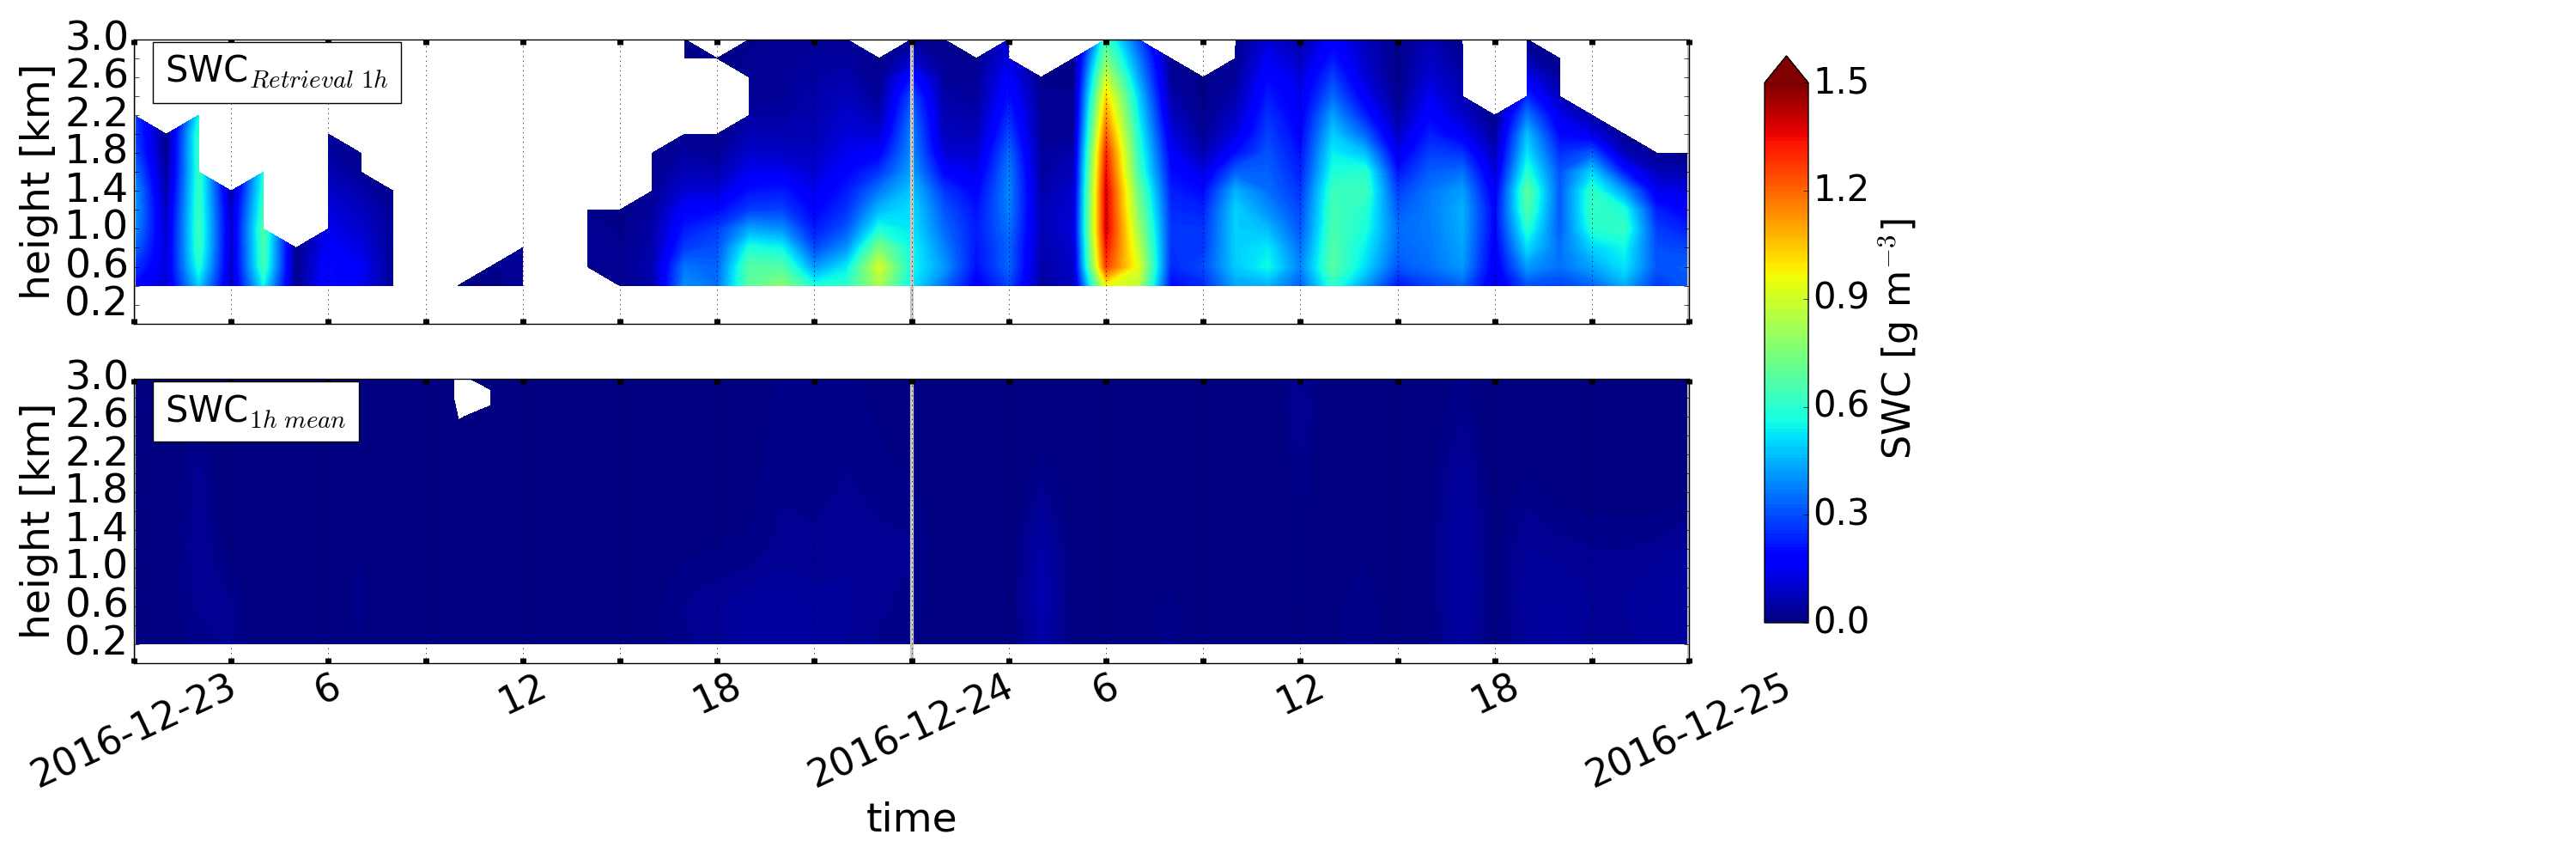
\includegraphics[trim={0.cm 0.8cm 19.cm 0.5cm},clip,width=0.9\textwidth]{./fig_vert_SWC_1h/20161223}
		\caption{}\label{fig:SWC1h:23}
	\end{subfigure}
	% 23/12
	\begin{subfigure}[t]{\textwidth}
		\centering
		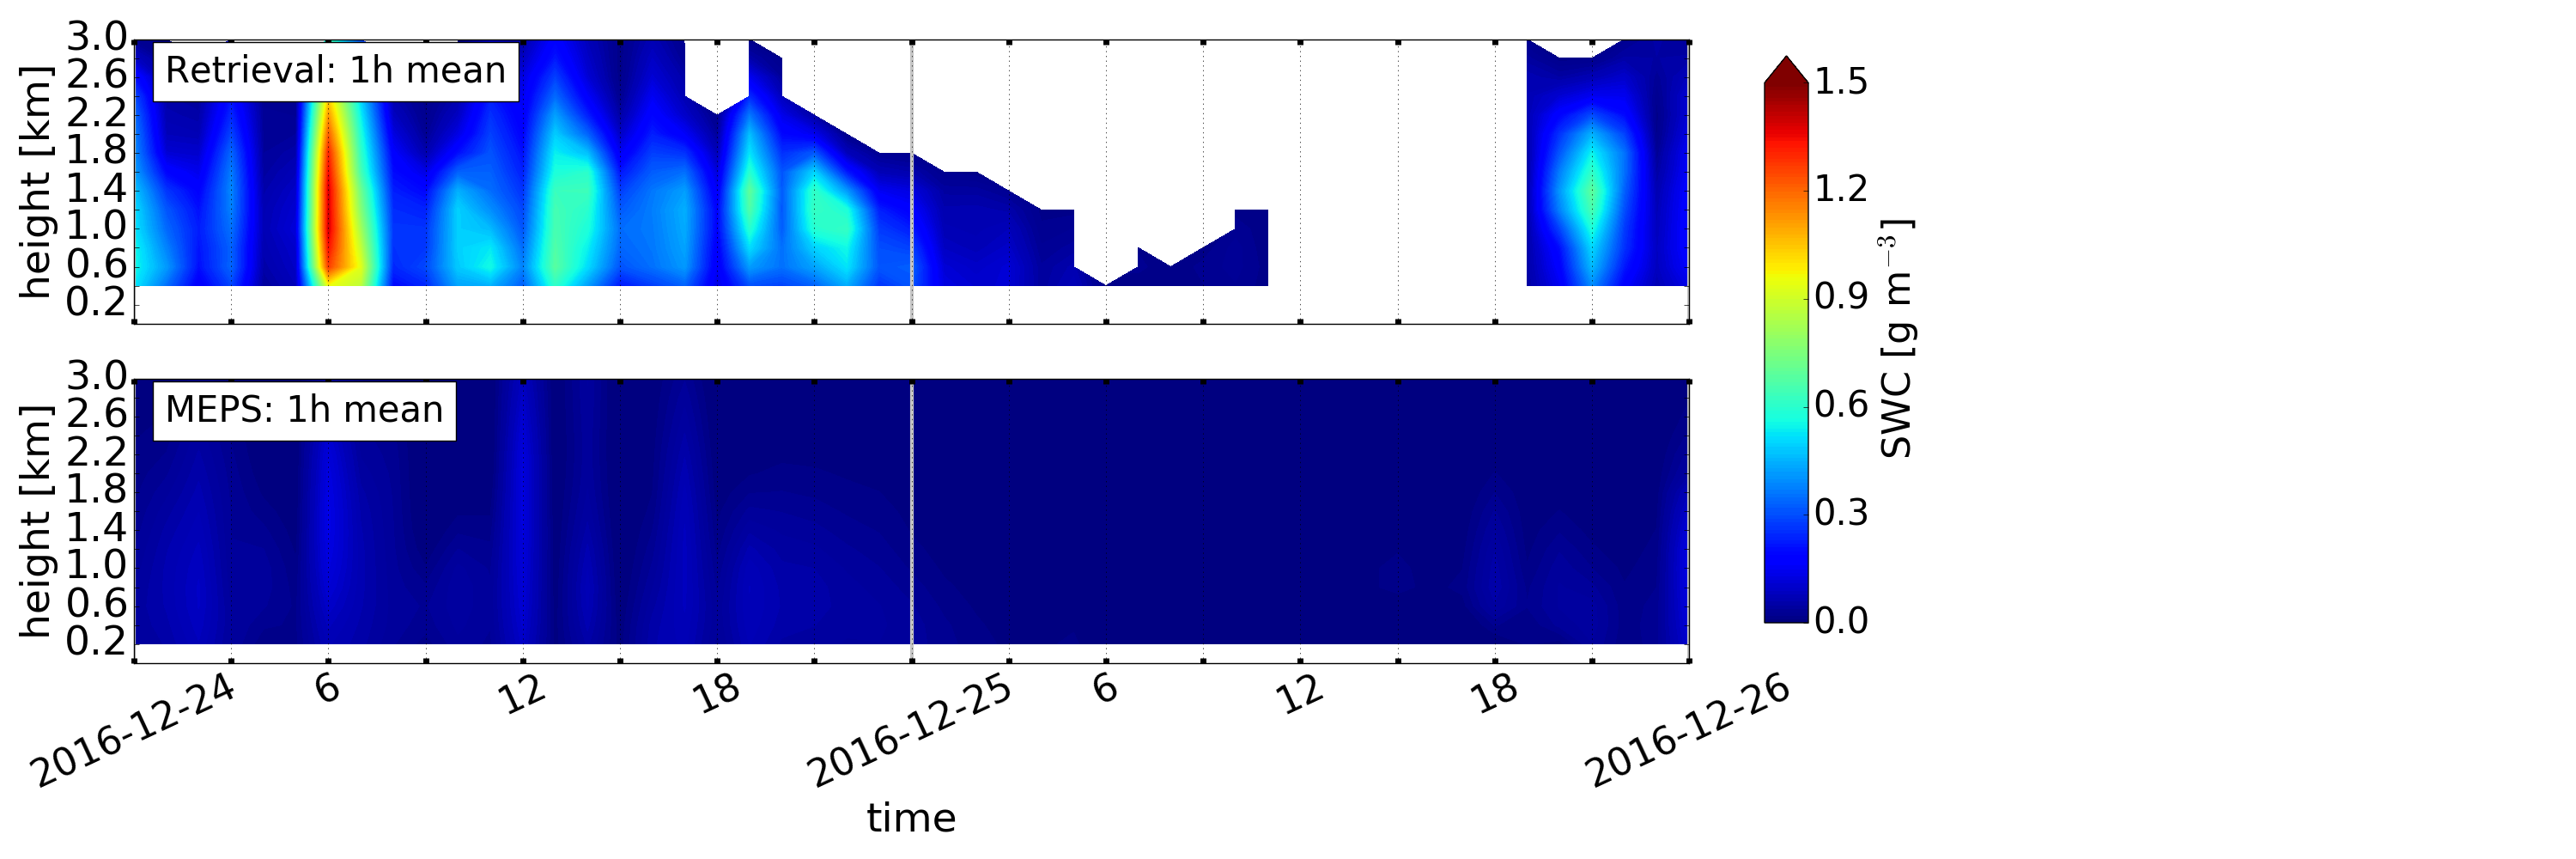
\includegraphics[trim={0.cm 0.8cm 19.cm 0.5cm},clip,width=0.9\textwidth]{./fig_vert_SWC_1h/20161224}
		\caption{}\label{fig:SWC1h:24}
	\end{subfigure}
	\caption{\textit{(Continued from previous page.)} Initialised \SIlist{23;24}{\dec} at \SI{0}{\UTC}.}
\end{figure}
\begin{figure}[t]\ContinuedFloat
	% 25/12
	\centering
	\begin{subfigure}[t]{\textwidth}
		\centering
		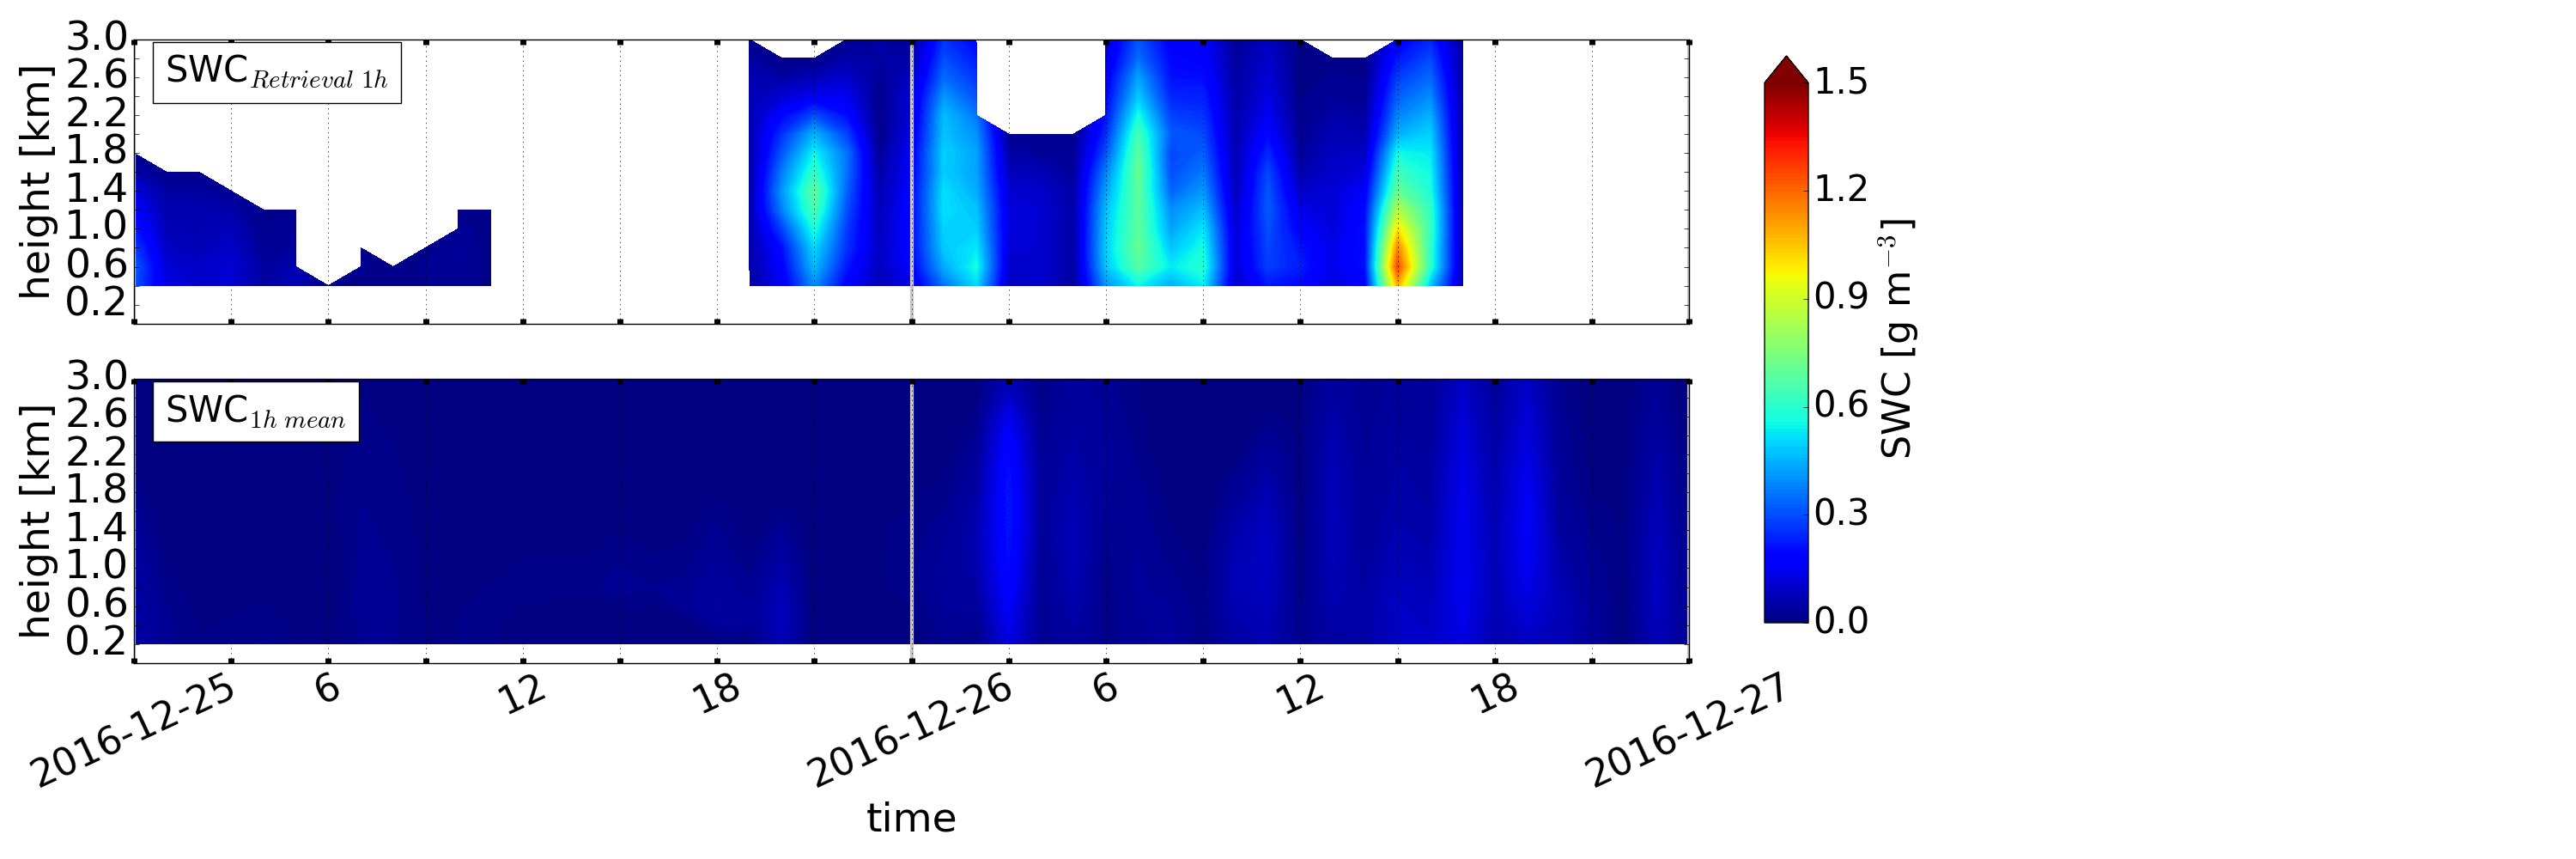
\includegraphics[trim={0.cm 0.8cm 19.cm 0.5cm},clip,width=0.9\textwidth]{./fig_vert_SWC_1h/20161225}
		\caption{}\label{fig:SWC1h:25}
	\end{subfigure}
	% \end{figure}
	% \begin{figure}[t]\ContinuedFloat
	% 	\centering
	% 26/12
	\begin{subfigure}[t]{\textwidth}
		\centering
		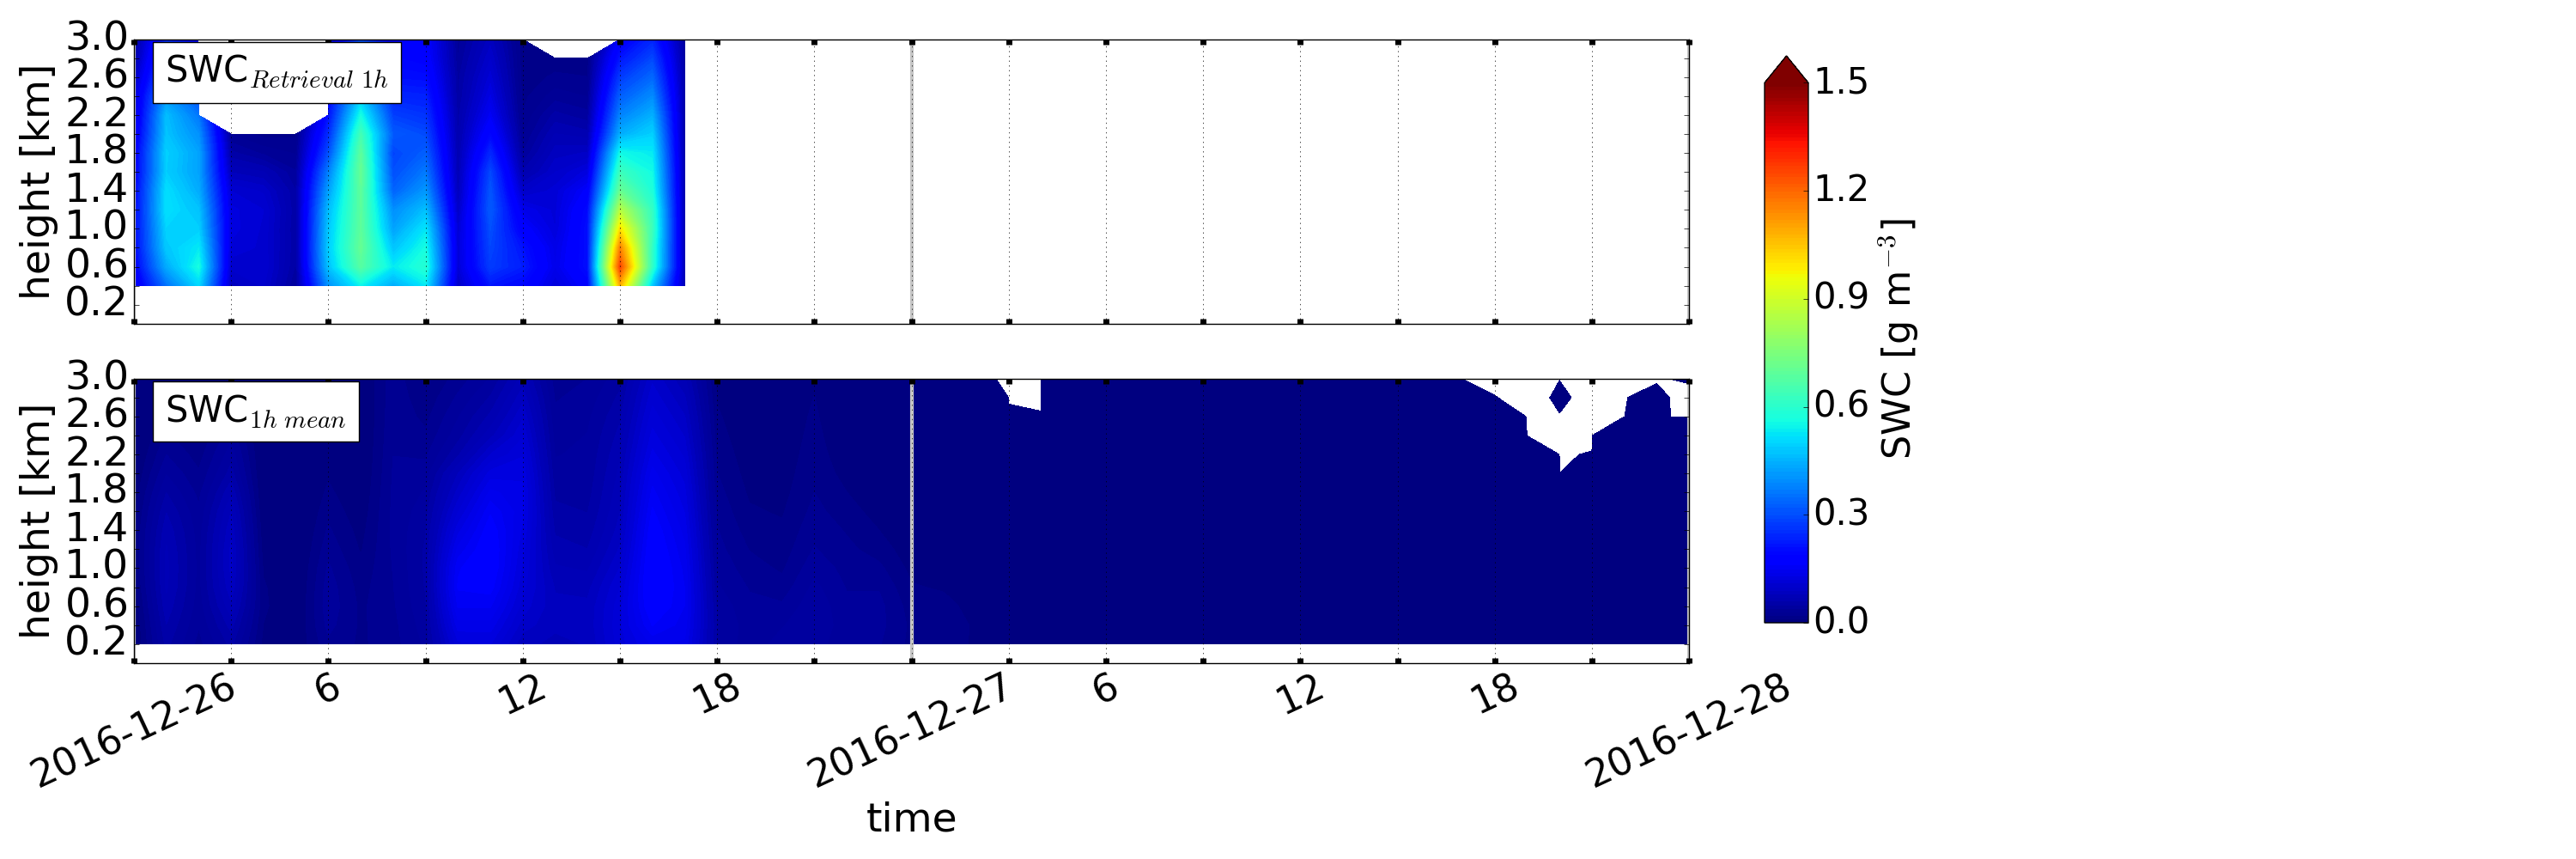
\includegraphics[trim={0.cm 0.8cm 19.cm 0.5cm},clip,width=0.9\textwidth]{./fig_vert_SWC_1h/20161226}
		\caption{}\label{fig:SWC1h:26}
	\end{subfigure}
	\caption{\textit{(Continued from previous page.)} Initialised \SIlist{25;26}{\dec} at \SI{0}{\UTC}.}   
\end{figure}
%%%%%%%%%%%%%%%%%%%%%%%%%%%%%%%%%%%%%%%%%%%%%%%%%%%%%%%%%%%%%%%%%%%%%%%%%%